\documentclass[12pt]{article}

% --- Packages ---
\usepackage{amsmath}        % math equations
\usepackage{amssymb}        % math symbols
\usepackage{graphicx}       % images/screenshots
\usepackage{listings}       % code blocks
\usepackage{xcolor}         % colors for code
\usepackage{geometry}       % page margins
\usepackage{hyperref}       % clickable links
\usepackage{enumitem}       % better lists
\usepackage{caption}
\usepackage{dirtree}

\geometry{margin=1in}
\setlength{\parindent}{0pt}
\setlength{\parskip}{6pt}

% --- Code styling ---
\lstset{
    language=Python,
    basicstyle=\ttfamily\small,
    keywordstyle=\color{blue},
    commentstyle=\color{gray},
    stringstyle=\color{orange},
    numbers=left,
    numberstyle=\tiny,
    breaklines=true,
    frame=single,
    backgroundcolor=\color{gray!10}
}

% --- Title ---
\title{RBE 500 -- Homework 2}
\author{Tracy}
\date{\today}

% ============================================================
\begin{document}
\maketitle
\tableofcontents
\newpage

% ============================================================
\section{Part 1: Problem Set}

% ----------
\textbf{Problem 2-35: Verify Equation (2.67).} 

\[
H^{-1} = 
\begin{bmatrix}
    R^T & -R^T d \\
    0 & 1 \\
\end{bmatrix}
\]

If $H = \begin{bmatrix} R & d \\ 0 & 1 \\ \end{bmatrix}$, we can verify its inverse Equation (2.67) 
by proving the dot product of the equations equals an identity matrix.
\begin{align*}
    H \cdot H^{-1} 
    &=
    \begin{bmatrix} R & d \\ 0 & 1 \end{bmatrix}
    \begin{bmatrix} R^T & -R^T d \\ 0 & 1 \end{bmatrix} \\
    &=
    \begin{bmatrix} RR^T & -RR^Td + d \\ 0 & 1 \end{bmatrix} \\
    &=
    \begin{bmatrix} I & 0 \\ 0 & 1 \end{bmatrix} \\
    &= I
\end{align*}

% ----------
\textbf{Problem 2-36: Compute the homogenous transformation representing a translation of 3 units along the x-axis 
followed by a rotation of $\frac{\pi}{2}$ about the current z-axis followed by a translation of 1 
unit along the fixed y-axis. Sketch the frame. What are the coordinates of the origin $o_1$ with
respect to the original frame in each case?} \\\\
While taking account of the order of matrix multiplication, current frames are post-multiplied and
fixed frames are pre-multiplied. With that, we have:
\[H = T_{y,1} \cdot T_{x,3} \cdot R_{z,\frac{\pi}{2}}\]

The individual matrices are:
\[
T_{x,3} = \begin{bmatrix}
    1 & 0 & 0 & 3\\
    0 & 1 & 0 & 0\\
    0 & 0 & 1 & 0\\
    0 & 0 & 0 & 1\\
\end{bmatrix}
\quad
R_{z,\frac{\pi}{2}} = \begin{bmatrix}
    0 & -1 & 0 & 0\\
    1 &  0 & 0 & 0\\
    0 &  0 & 1 & 0\\
    0 &  0 & 0 & 1\\
\end{bmatrix}
\quad
T_{y,1} = \begin{bmatrix}
    1 & 0 & 0 & 0\\
    0 & 1 & 0 & 1\\
    0 & 0 & 1 & 0\\
    0 & 0 & 0 & 1\\
\end{bmatrix}
\]

Computing $T_{x,3} \cdot R_{z,\frac{\pi}{2}}$:
\[
T_{x,3} \cdot R_{z,\frac{\pi}{2}} = \begin{bmatrix}
    0 & -1 & 0 & 3\\
    1 &  0 & 0 & 0\\
    0 &  0 & 1 & 0\\
    0 &  0 & 0 & 1\\
\end{bmatrix}
\]

Then pre-multiplying by $T_{y,1}$:
\[
H = \begin{bmatrix}
    0 & -1 & 0 & 3\\
    1 &  0 & 0 & 1\\
    0 &  0 & 1 & 0\\
    0 &  0 & 0 & 1\\
\end{bmatrix}
\]

The origin $o_1$ expressed in the base frame is the translation vector (last column):
\[
o_1 = \begin{bmatrix} 3 \\ 1 \\ 0 \end{bmatrix}
\]

% ----------
\textbf{Problem 2-37: Consider the diagram of Figure 2.13. Find the homogenous transformations $H_1^0$ $H_2^0$ $H_2^1$
representing the transformations among the three frames shown. Show that $H_2^0 = H_1^0, H_2^1$.} \\\\

\begin{figure}[htbp]
    \centering
    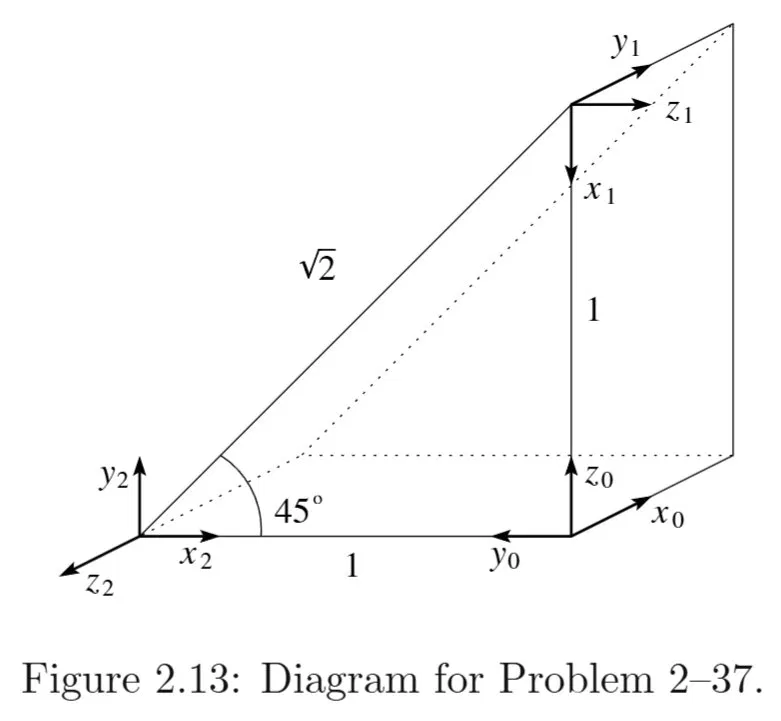
\includegraphics[width=0.3\textwidth]{screenshots/fig2_13.png}
    \label{fig:fig2.13}
\end{figure}

\textbf{Frame 1} is 1 unit above Frame 0 along $z_0$, with axes:
$x_1 = -z_0$, $y_1 = y_0$, $z_1 = x_0$.

\textbf{Frame 2} is 1 unit along $y_0$ from the origin, with axes:
$x_2 = -y_0$, $y_2 = z_0$, $z_2 = -x_0$.

\[
H_1^0 = 
\begin{bmatrix}
 0 & 0 & 1 & 0 \\
 0 & 1 & 0 & 0 \\
-1 & 0 & 0 & 1 \\
 0 & 0 & 0 & 1
\end{bmatrix}
\quad
H_2^0 = 
\begin{bmatrix}
 0 &  0 & -1 & 0 \\
-1 &  0 &  0 & 1 \\
 0 &  1 &  0 & 0 \\
 0 &  0 &  0 & 1
\end{bmatrix}
\]

\textbf{Inverse of $H_1^0$:}
\[
(H_1^0)^{-1} = 
\begin{bmatrix}
 0 & 0 & -1 & -1 \\
 0 & 1 &  0 &  0 \\
 1 & 0 &  0 &  0 \\
 0 & 0 &  0 &  1
\end{bmatrix}
\]

\textbf{Transformation $H_2^1$:}
\[
\begin{align*}
    H_2^1 &= (H_1^0)^{-1} \cdot H_2^0\\
    &=
    \begin{bmatrix}
        0 & 0 & -1 & -1\\
        0 & 1 &  0 &  0\\
        1 & 0 &  0 &  0\\
        0 & 0 &  0 &  1\\
    \end{bmatrix}
    \begin{bmatrix}
         0 & 0 & -1 & 0\\
        -1 & 0 &  0 & 1\\
         0 & 1 &  0 & 0\\
         0 & 0 &  0 & 1\\
    \end{bmatrix}\\
    &=
    \begin{bmatrix}
         0 & -1 &  0 & -1\\
        -1 &  0 &  0 &  1\\
         0 &  0 & -1 &  0\\
         0 &  0 &  0 &  1\\
    \end{bmatrix}\\
\end{align*}
\]

% ----------
\textbf{Problem 2-38: Consider the diagram of Figure 2.14. A robot is set up 1 meter from a table. The table top is 1
meter high an 1 meter square. A frame $o_1 x_1 y_1 z_1$ is fixed to the edge of the table as shown.
A cube measuring 20 cm on a side is placed in the center of the table with frame $o_2 x_2 y_2 z_2$
established at the center of the cube as shown. A camera is situated directly above the center of
the block 2 meters above the table top with frame $o_3 x_3 y_3 z_3$ attached as shown. Find the
homogenous transformation relating the frame $o_2 x_2 y_2 z_2$ to the camera frame $o_3 x_3 y_3 z_3$.} \\\\

\begin{figure}[htbp]
    \centering
    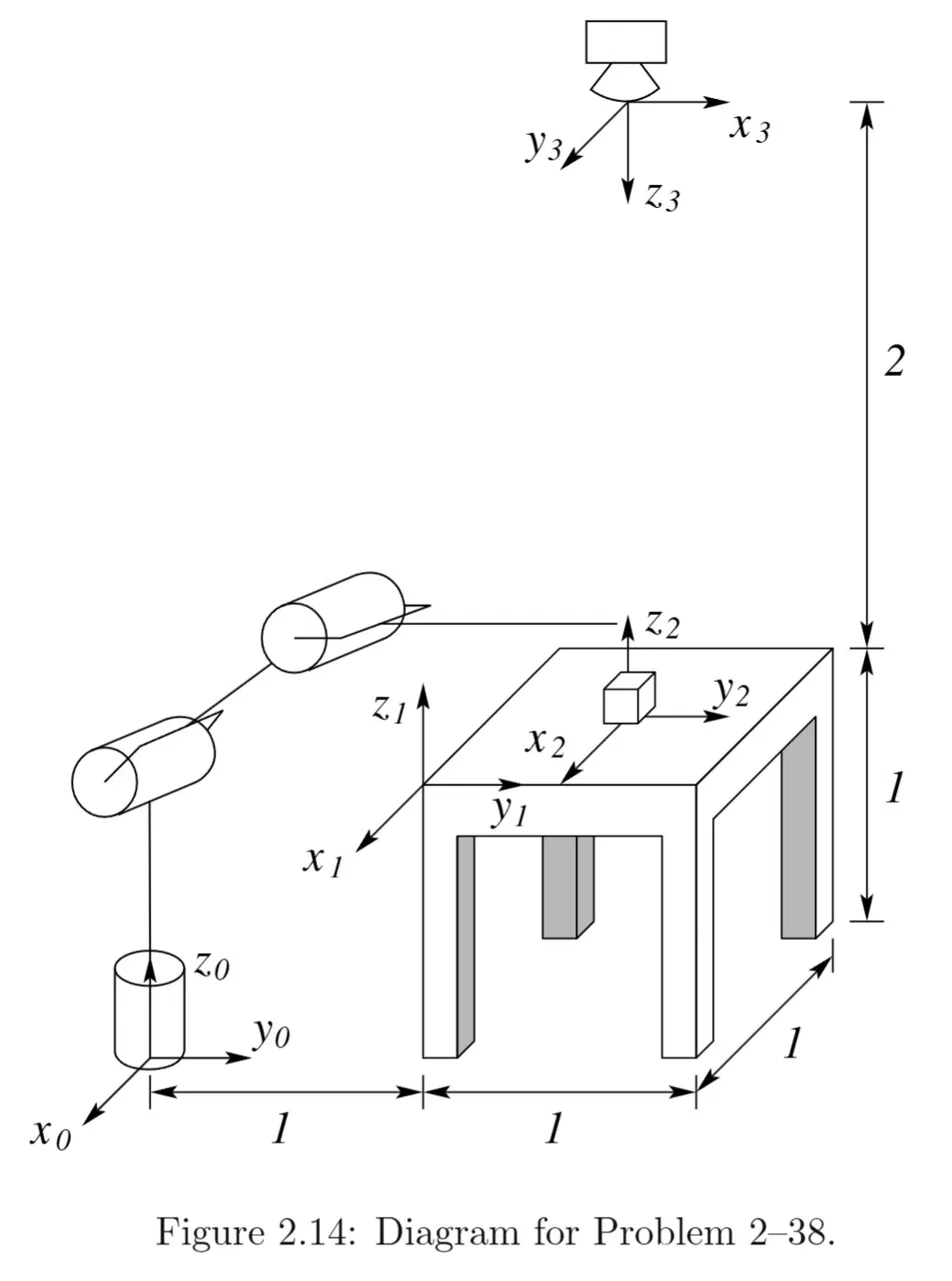
\includegraphics[width=0.4\textwidth]{screenshots/fig2_14.png}
    \label{fig:fig2.14}
\end{figure}

From Figure 2.14, we identify the following frames relative
to Frame 0 (robot base). The robot is 1m from the table edge, the table
is 1m high and 1m square, the cube is 20cm on a side (so its center is
0.1m above the table), and the camera is 2m above the table top.

\begin{itemize}
    \item Frame 1: table edge, translated 1m along $y_0$ and 1m up
    along $z_0$, same orientation as Frame 0
    \item Frame 2: cube center, offset $-0.5$m along $x_0$, 1.5m along
    $y_0$, and 1.1m along $z_0$ (1m table + 0.1m half-cube height),
    same orientation as Frame 0
    \item Frame 3: camera, directly above cube center at 3m height,
    same orientation as Frame 0
\end{itemize}

\textbf{Homogeneous transformations relative to Frame 0:}
\[
H_1^0 = 
\begin{bmatrix}
1 & 0 & 0 & 0 \\
0 & 1 & 0 & 1 \\
0 & 0 & 1 & 1 \\
0 & 0 & 0 & 1
\end{bmatrix}
\quad
H_2^0 = 
\begin{bmatrix}
1 & 0 & 0 & -0.5 \\
0 & 1 & 0 &  1.5 \\
0 & 0 & 1 &  1.1 \\
0 & 0 & 0 &    1
\end{bmatrix}
\quad
H_3^0 = 
\begin{bmatrix}
1 & 0 & 0 & -0.5 \\
0 & 1 & 0 &  1.5 \\
0 & 0 & 1 &    3 \\
0 & 0 & 0 &    1
\end{bmatrix}
\]

\textbf{Finding $H_2^3 = (H_3^0)^{-1} \cdot H_2^0$:}

Since Frame 3 has no rotation relative to Frame 0 (i.e.\ $R_3^0 = I$),
the inverse simplifies to:
\[
(H_3^0)^{-1} = \begin{bmatrix}
1 & 0 & 0 &  0.5 \\
0 & 1 & 0 & -1.5 \\
0 & 0 & 1 &   -3 \\
0 & 0 & 0 &    1
\end{bmatrix}
\]

\[
H_2^3 = (H_3^0)^{-1} \cdot H_2^0 =
\begin{bmatrix} 1 & 0 & 0 & 0.5\\ 0 & 1 & 0 & -1.5\\ 0 & 0 & 1 & -3\\ 0 & 0 & 0 & 1\end{bmatrix}
\begin{bmatrix} 1 & 0 & 0 & -0.5\\ 0 & 1 & 0 & 1.5\\ 0 & 0 & 1 & 1.1\\ 0 & 0 & 0 & 1\end{bmatrix}
=
\begin{bmatrix} 1 & 0 & 0 & 0\\ 0 & 1 & 0 & 0\\ 0 & 0 & 1 & -1.9\\ 0 & 0 & 0 & 1\end{bmatrix}
\]

The translation vector $(0, 0, 1.9)^T$ confirms that the cube center lies directly below the camera
at a distance of $2 - 0.1 = 1.9$ meters, which is consistent with the geometry in Figure 2.14.\\

% ----------
\textbf{Problem 2-42: In general, multiplication of homogenous transformation matrices is not commutative. Consider the
matrix product\[ H = R_{x,\alpha} \cdot T_{x,b} \cdot T_{z,d} \cdot R_{z,\theta} \]
Determine which pairs of the four matrices on the right-hand side commute. Explain why these pairs
commute. Find all permutations of these four matrices that yield the same homogenous transformation
matrix, $H$.} \\\\

The four matrices are:
\[
R_{x,\alpha} = 
\begin{bmatrix}
    1 &        0 &         0 & 0\\
    0 & c_\alpha & -s_\alpha & 0\\
    0 & s_\alpha &  c_\alpha & 0\\
    0 &        0 &         0 & 1
\end{bmatrix}, 
\quad
T_{x,b} = 
\begin{bmatrix}
    1 & 0 & 0 & b\\
    0 & 1 & 0 & 0\\
    0 & 0 & 1 & 0\\
    0 & 0 & 0 & 1
\end{bmatrix}
\]
\[
T_{z,d} = 
\begin{bmatrix}
    1 & 0 & 0 & 0\\
    0 & 1 & 0 & 0\\
    0 & 0 & 1 & d\\
    0 & 0 & 0 & 1
\end{bmatrix}, 
\quad
R_{z,\theta} = 
\begin{bmatrix}
    c_\theta & -s_\theta & 0 & 0\\
    s_\theta &  c_\theta & 0 & 0\\
           0 &         0 & 1 & 0\\
           0 &         0 & 0 & 1
\end{bmatrix}
\]

\textbf{Commuting Pairs:}

\begin{itemize}
    \item $R_{x,\alpha}$ and $T_{x,b}$ \textbf{commute}: a rotation about
    the $x$-axis and a translation along the $x$-axis act independently.
    \item $T_{x,b}$ and $T_{z,d}$ \textbf{commute}: pure translations
    always commute regardless of direction.
    \item $T_{z,d}$ and $R_{z,\theta}$ \textbf{commute}: a translation
    along the $z$-axis and a rotation about the $z$-axis act independently.
    \item All other pairs \textbf{do not commute}.
\end{itemize}

\textbf{Valid Permutations:}

Using the commuting pairs to swap neighbors, the following permutations
all yield the same $H$:

\begin{enumerate}
    \item $R_{x,\alpha} \cdot T_{x,b} \cdot T_{z,d} \cdot R_{z,\theta}$
    \item $T_{x,b} \cdot R_{x,\alpha} \cdot T_{z,d} \cdot R_{z,\theta}$
    \item $R_{x,\alpha} \cdot T_{x,b} \cdot R_{z,\theta} \cdot T_{z,d}$
    \item $T_{x,b} \cdot R_{x,\alpha} \cdot R_{z,\theta} \cdot T_{z,d}$
    \item $R_{x,\alpha} \cdot T_{z,d} \cdot T_{x,b} \cdot R_{z,\theta}$
\end{enumerate}
\newpage

% ============================================================
\section{Part 2: ROS 2 Assignment}

\subsection{Overview}
Brief description of what the node does.

\subsection{Package Structure}
\dirtree{%
    .1 quat\_to\_euler/.
    .2 quat\_to\_euler/.
    .3 \_\_init\_\_.py.
    .3 quat\_to\_euler\_node.py.
    .2 package.xml.
    .2 setup.py.
    .2 setup.cfg.
}

\subsection{Node Implementation}

\begin{lstlisting}
# Paste your Python code here
import rclpy
from rclpy.node import Node
...
\end{lstlisting}

\subsection{Conversion Formulas}

The quaternion $(w, x, y, z)$ is converted to Euler angles $(\phi, \theta, \psi)$ using:

\begin{align}
\phi   &= \arctan2\!\left(2(wx + yz),\; 1 - 2(x^2 + y^2)\right) \\
\theta &= \arcsin\!\left(2(wy - zx)\right) \\
\psi   &= \arctan2\!\left(2(wz + xy),\; 1 - 2(y^2 + z^2)\right)
\end{align}

\subsection{How to Run}

\begin{verbatim}
ros2 run quat_to_euler quat_to_euler_node
\end{verbatim}

Publish a test quaternion from the terminal:
\begin{verbatim}
ros2 topic pub /quaternion std_msgs/msg/Float32MultiArray \
  "data: [1.0, 0.0, 0.0, 0.0]"
\end{verbatim}

\subsection{Results}

% To include a screenshot:
% \begin{figure}[h]
%     \centering
%     \includegraphics[width=0.8\textwidth]{screenshot.png}
%     \caption{Terminal output showing Euler angle conversion}
% \end{figure}

\end{document}